\documentclass[signature=data]{physicsreport}
\usepackage{graphicx}

%%
%% User settings
%%

\classno{}
\stuno{}
\groupno{}
\stuname{}
\expdate{\expdatefmt\today}
\expname{磁耦合共振式无线电力传输实验(后半)}

%%
%% Document body
%%

\begin{document}
% First page
% Some titles and personal information are defined in ``\maketitle''.
\maketitle

\section{实验预习指导}
\newpage

\section{原始数据记录}
% Teacher signature
\makeatletter
\physicsreport@body@signature{data}
\makeatother

\newpage

% Data process and others
\section{数据处理}
\subsection{研究振荡频率对电力传输效率的影响}
绘制幅度-频率曲线,总结曲线规律。
\begin{figure}[htbp]
    \centering
    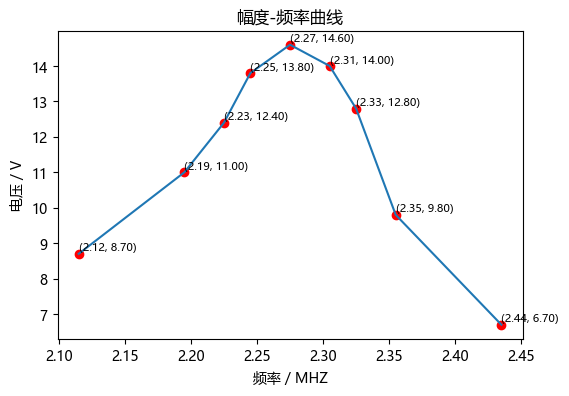
\includegraphics[width=7cm]{images/lab7/output.png}
    \caption{幅度-频率曲线}
\end{figure}

当频率处于共振频率时,电压幅值最高,电力传输效率最高。频率与共振频率的差值越大,电压幅值越低。

\subsection{研究无线电力传输的距离对传输效果影响}
绘制灯泡电压-距离曲线,总结曲线规律。
\begin{figure}[htbp]
    \centering
    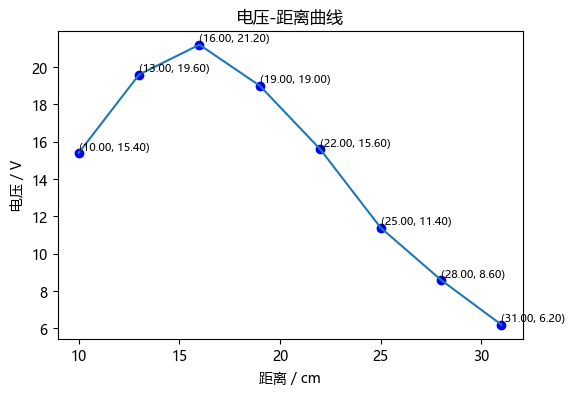
\includegraphics[width=7cm]{images/lab7/output2.png}
    \caption{电压-距离曲线}
\end{figure}

灯泡电压随距离的增大,先增大后减小,在$16cm$左右出现最大值。

\vspace{1em}

\subsection{自制无线电力传输系统}
总结实际传输效果,分析误差产生的原因。

自制线圈的实际最远传输距离为$12.5cm$,理论共振频率和实际共振频率基本符合。传输效果较好。

可能原因:线圈的匝数和尺寸不够精确,两线圈的电容值因制作工艺等原因存在一定差值。
\newpage

\section{讨论题}
\subsection{为什么当振荡频率和LC电路的频率一样时,发射线圈能在周围产生大的交变磁场?}
当振荡频率与LC电路的固有频率一致时,即共振频率,发射线圈会处于共振状态。电源电压的变化频率与电容、电感之间相互充放电的频率一致。在共振状态下,电路中的电流和电压会达到最大值,并且能量在电感和电容之间来回振荡。
\vspace{2em}
\subsection{你认为提高磁耦合谐振式无线电力传输系统能量传输效率的方式有哪些?}

在发射线圈和接收线圈之间增加一个线圈,通过精确控制电路参数和频率源,提高系统的共振频率精度,优化线圈的匝数、尺寸。
\end{document}